Android Studio ist eine vom Andoid Open Source Project (kurz: AOSP) entwickelte Entwicklungsumgebung auf der basis von IntelliJ, dabei sollte beachtet werden, dass Android Studio im gegensatz zu Android OS
proprietären Code beinhaltet und somit weder open source ist, noch ohne erlaubnis durch dritte weiterverbreitet werden darf.
IntelliJ ist eine bereits bestehende propietäre Entwicklungsumgebung für Java (bzw. JVM) und Android, des weiteren kann eine Lizenz für Firmen und Webentwickler erworben werden.
Im grunde wurde Android Studio mit der hinsicht auf Applikationsentwicklung auf dem Android OS erstellt. Es beinhaltet von Haus aus notwendige, aber auch arbeitserleichternde Komponenten, wie
einen Gradle-Compiler (Notwendig) oder einen Android-Empulator (Erleichtert das testen der App auf einem Computer).\\

%FIXME rechtschreibung
Gradle ist ein Open Source Build-Tool, was im Grunde über den eigentlichen Compiler-Prgogrammen eine oberste Schicht in der Compiler-Toolchain bildet. Daher verkörpert Gradle mehrere separate aufgaben in sich und vereinfacht das kompillieren von Android Apps enorm.
Die Kernkompnenten von Gradle sind
\begin{itemize}
\item \textbf{Linker, bzw. Zusammentragen von zusätzlichen Paketen und androidspezifischen Dateien, die für das Kompillieren erforderlich sind.} Dabei werden Pakete resp. Bibliotheken von den Quellen runtergeladen, 
die man zu der Quellenliste hinzugefügt hat. Dies erleichtert das Hinzufügen von Bibliotheken wie z.B. einer Bibliothek zum herunterladen und anzeigen von Bildern, da man nur die Downloadadresse angeben muss
und sich nicht mehr um das Einbinden der Bibliothek in sein Applikationsprojekt kümmern muss.

\item \textbf{Debugger} Wie bereits beschrieben liest sich der Debugger noch vor dem Precompiler den Code durch und macht den Programmierer auf allfällige Fehler oder verbesserungen aufmerksam.

\item \textbf{Precompiler} Der Precompiler ist ein Kernbestandteil der Compiler-Toolchain. Eine Toolchain ist eine Ansammlung von Programmen, die einem helfen aus geschriebenen Code und Assets ein lauffähiges
Programm zu erstellen. Er liest jede Datei durch und bereitet sie auf die nachfolgenden Verarbeitungsprozesse vor, indem er unter anderem Kommentare entfernt, nichtgenutzte Funktionen und Variabeln entfernt, Makros ersetzt und durch die \verb include -Kontrollzequenz eingebundene Dateien einfügt. Die heutigen Precompiler bleiben aber meist nicht nur bei ihren Kernaufgaben, sondern versuchen auch den Code so weit zu verbessern,
dass er nach dem Kompilliervorgang eine geringere Laufzeit und Speicheraulastung aufweist. Dabei ist aber zu beachten dass Compiler und Precompiler sehr eng miteinander zusammenarbeiten.

\item \textbf{Compiler} Der Compiler ist wohl das bekannteste Programm aus einer klassischen Toolchain. Er sogt dafür, dass die von dem Precompiler aufbereiteten Dateien in Maschinensprache übersetzt werden.
Wie bereits in der Einleitung erwähnt rechnet der Computer Binär. Daher ist eine Datei nichts anderes als eine lange Zahl. Je nach Prozessortyp wird auch eine Zahl anders verarbeitet. Dieser unterschied liegt in der verarbeitung von Kontrollsequenzen. In diesem trivialen Beispiel soll verdeutlicht werden, wie zwei verschiedene Prozessoren ein und die selbe Zahl anders interpretieren: Der Befehl für eine additionsoperation wird hier durch 11100010 repräsentiert. Im Prozessortyp A löst dies wie gewollt eine Addition aus, hingegen im Prozessortyp B werden die nachfolgenden Bits in den Zwischenspeicher kopiert. Prozessoren haben also auch ihre eigene Sprache, die sich durch ihre Herstellung ergibt. Diese Sprache wird \textit{Befehlssatz} genannt, wohingegen der Prozessortyp \textit{Architektur} genannt wird. Jede Prozessorarchitektur hat ihren eigenen Compiler.
Im Fall von Android haben sich drei Architekturen etabiliert: armeabi-v7, Intel x86 und AMD64. Die App wird also in mehrere Sprachen übersetzt bevor sie ausgeleifert wird.
\end{itemize}

\newpage

\begin{figure}[htbp] 
  \centering
     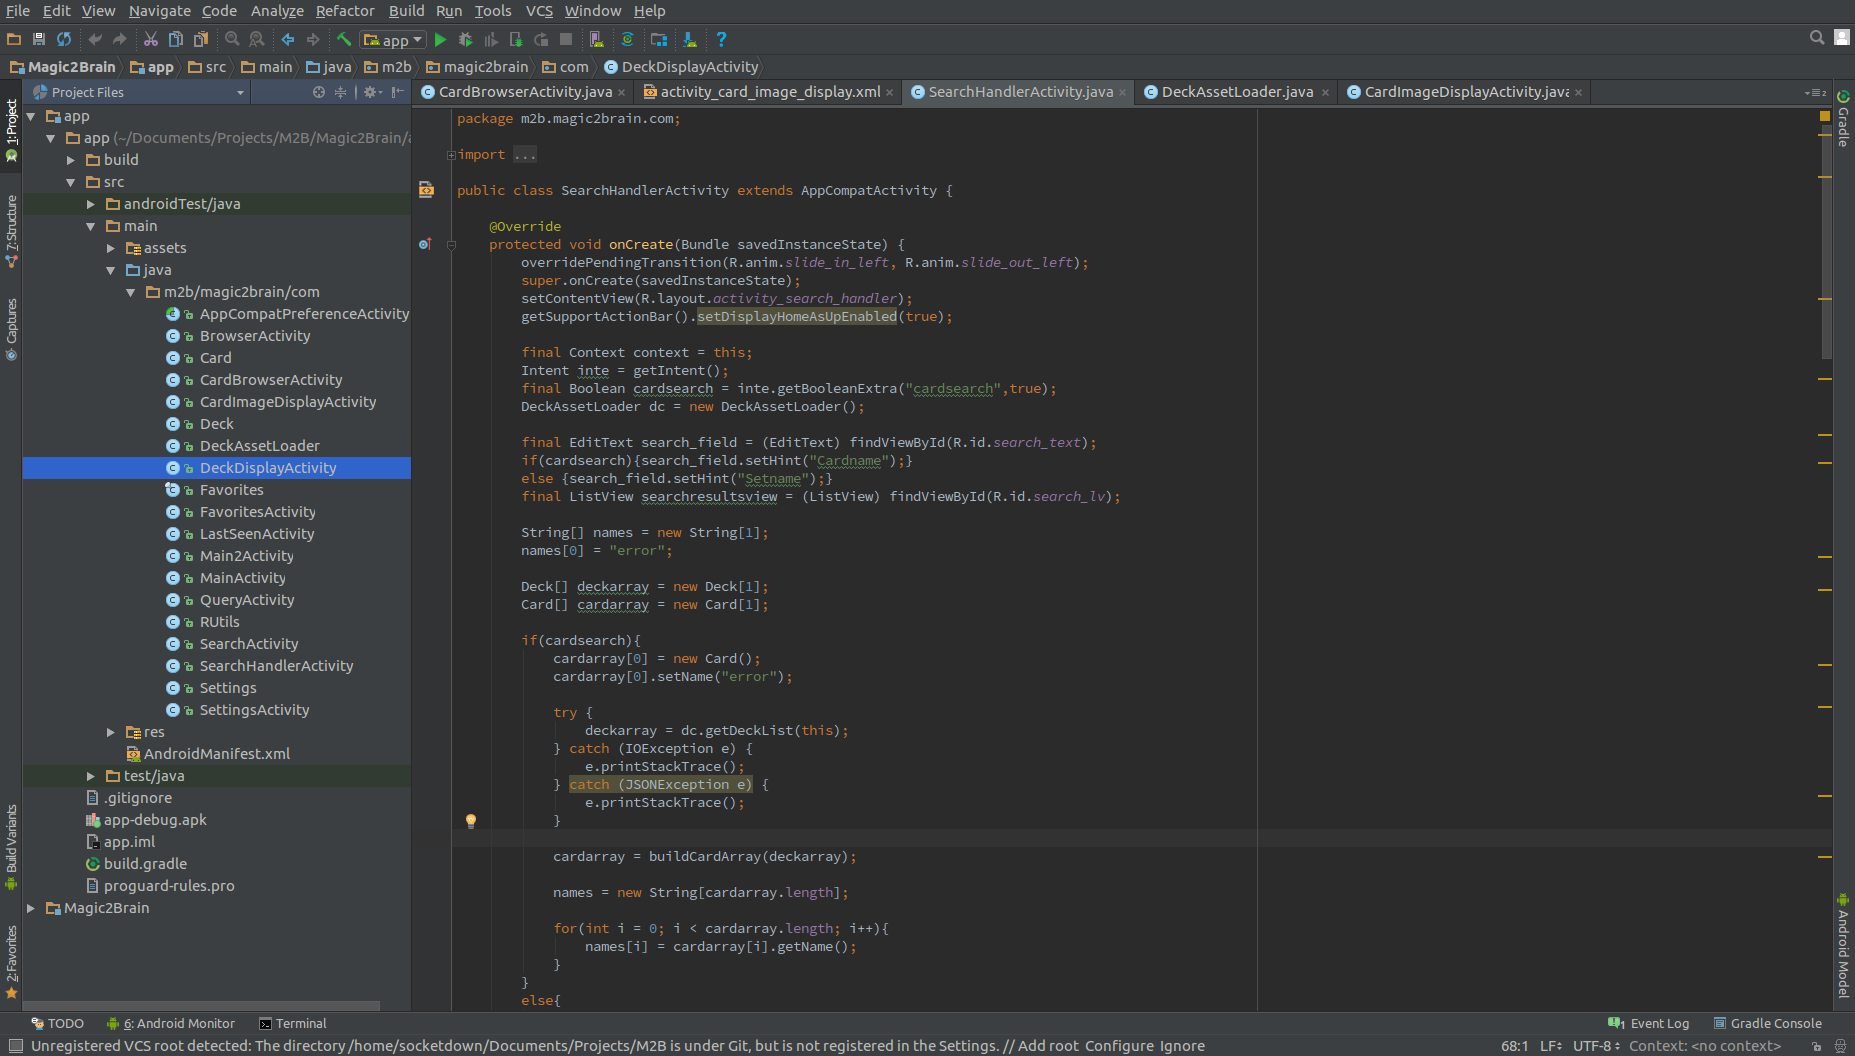
\includegraphics[width=1\textwidth]{AndroidStudio_GUI.png}
  \caption{Android Studio Benutzeroberfläche \cite{ASGUI}}
  \label{fig:Android Studio GUI}
\end{figure}
Die Grafische Benutzeroberfläche ist das Wichtigste an einer IDE. Sie erleichtert dem Entwickler die Navigation durch seinen Code in Form von Farbmarkierungen (Rechts) und Dateibrowser (Links).
Die Toolbar von Android Studio (Oben) ist mit wichtigen Shortcuts, wie z.B. Kompillierung starten, Emulator starten und Android SDK aktualisieren, gefüllt.

%TODO ASGUI fertigschreiben